\exercisesheader{}

% 1

\eoce{\qt{True or false\label{tf_prob_definitions}} Determine if the statements 
below are true or false, and explain your reasoning.
\begin{parts}
\item If a fair coin is tossed many times and the last eight tosses are all heads, 
then the chance that the next toss will be heads is somewhat less than 50\%.
\item Drawing a face card (jack, queen, or king) and drawing a red card from a 
full deck of playing cards are mutually exclusive events.
\item Drawing a face card and drawing an ace from a full deck of playing cards 
are mutually exclusive events.
\end{parts}
}{}

% 2

\eoce{\qt{Roulette wheel\label{roulette_wheel}} The game of roulette involves 
spinning a wheel with 38 slots: 18 red, 18 black, and 2 green. A ball is spun 
onto the wheel and will eventually land in a slot, where each slot has an equal 
chance of capturing the ball.

\noindent%
\begin{minipage}[c]{0.65\textwidth}
\raggedright\begin{parts}
\item You watch a roulette wheel spin 3 consecutive times and the ball lands on a 
red slot each time. What is the probability that the ball will land on a red slot 
on the next spin?
\item You watch a roulette wheel spin 300 consecutive times and the ball lands on 
a red slot each time. What is the probability that the ball will land on a red 
slot on the next spin?
\item Are you equally confident of your answers to parts~(a) and~(b)? Why or why 
not?
\end{parts}
\end{minipage}
\begin{minipage}[c]{0.05\textwidth}
\ 
\end{minipage}
\begin{minipage}[c]{0.28\textwidth}
\begin{center}
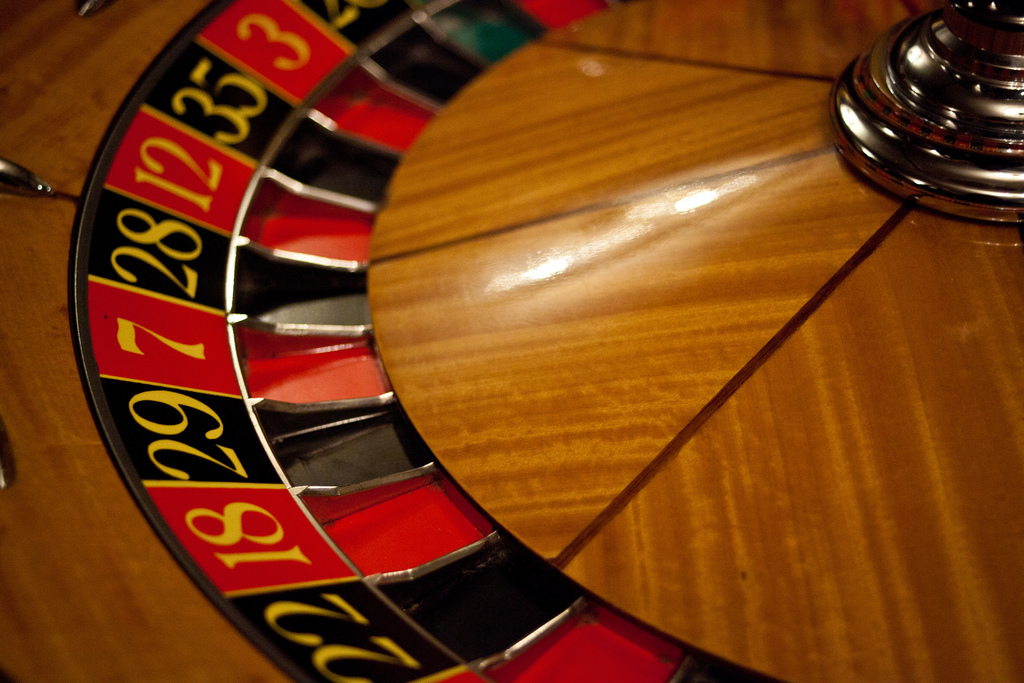
\includegraphics[width = \textwidth]{ch_probability/figures/eoce/roulette_wheel/roulette_wheel.jpg} \\
{\footnotesize Photo by H\r{a}kan Dahlstr\"{o}m \\
  (\oiRedirect{textbook-flickr_hakan_dahlstrom_roulette_wheel}{http://flic.kr/p/93fEzp}) \\
  \oiRedirect{textbook-CC_BY_2}{CC~BY~2.0~license}}
\end{center}
\end{minipage}
}{}

% 3

\eoce{\qt{Four games, one winner\label{four_games_one_winner}} Below are four 
versions of the same game. Your archnemesis gets to pick the version of the game, 
and then you get to choose how many times to flip a coin: 10 times or 100 times. 
Identify how many coin flips you should choose for each version of the game. It 
costs \$1 to play each game. Explain your reasoning.
\begin{parts}
\item If the proportion of heads is larger than 0.60, you win \$1.
\item If the proportion of heads is larger than 0.40, you win \$1.
\item If the proportion of heads is between 0.40 and 0.60, you win \$1.
\item If the proportion of heads is smaller than 0.30, you win \$1.
\end{parts}
}{}

% 4

\eoce{\qt{Backgammon\label{backgammon}} Backgammon is a board game for two 
players in which the playing pieces are moved according to the roll of two dice. 
Players win by removing all of their pieces from the board, so it is usually good 
to roll high numbers. You are playing backgammon with a friend and you roll two 
6s in your first roll and two 6s in your second roll. Your friend rolls two 3s in 
his first roll and again in his second row. Your friend claims that you are 
cheating, because rolling double 6s twice in a row is very unlikely. Using 
probability, show that your rolls were just as likely as~his.
}{}

% 5

\eoce{\qt{Coin flips\label{coin_flips}} If you flip a fair coin 10 times, what is 
the probability of
\begin{parts}
\item getting all tails? 
\item getting all heads? 
\item getting at least one tails? 
\end{parts}
}{}

% 6

\eoce{\qt{Dice rolls\label{dice_rolls}} If you roll a pair of fair dice, what is 
the probability of
\begin{parts}
\item getting a sum of 1?
\item getting a sum of 5?
\item getting a sum of 12?
\end{parts}
}{}

% 7

\eoce{\qt{Swing voters\label{swing_voters}} A Pew Research survey asked 2,373 
randomly sampled registered voters their political affiliation (Republican, 
Democrat, or Independent) and whether or not they identify as swing voters. 35\% 
of respondents identified as Independent, 23\% identified as swing voters, and 
11\% identified as both.\footfullcite{indepSwing}
\begin{parts}
\item Are being Independent and being a swing voter disjoint, i.e. mutually 
exclusive?
\item Draw a Venn diagram summarizing the variables and their associated 
probabilities.
\item What percent of voters are Independent but not swing voters?
\item What percent of voters are Independent or swing voters?
\item What percent of voters are neither Independent nor swing voters?
\item Is the event that someone is a swing voter independent of the event that 
someone is a political Independent?
\end{parts}
}{}

% 8

\eoce{\qt{Poverty and language\label{poverty_language}} The American Community 
Survey is an ongoing survey that provides data every year to give communities the 
current information they need to plan investments and services. The 2010 American 
Community Survey estimates that 14.6\% of Americans live below the poverty line, 
20.7\% speak a language other than English (foreign language) at home, and 4.2\% 
fall into both categories. \footfullcite{poorLang}
\begin{parts}
\item Are living below the poverty line and speaking a foreign language at home 
disjoint?
\item Draw a Venn diagram summarizing the variables and their associated 
probabilities.
\item What percent of Americans live below the poverty line and only speak 
English at home?
\item What percent of Americans live below the poverty line or speak a foreign 
language at home?
\item What percent of Americans live above the poverty line and only speak 
English at home? 
\item Is the event that someone lives below the poverty line independent of the 
event that the person speaks a foreign language at home?
\end{parts}
}{}

% 9

\eoce{\qt{Disjoint vs. independent\label{disjoint_indep}} In parts~(a) and~(b), 
identify whether the events are disjoint, independent, or neither (events cannot 
be both disjoint and independent).
\begin{parts}
\item You and a randomly selected student from your class both earn A's in this 
course. 
\item You and your class study partner both earn A's in this course.
\item If two events can occur at the same time, must they be dependent?
\end{parts}
}{}

% 10

\eoce{\qt{Guessing on an exam\label{guessing_on_exam}} In a multiple choice exam, 
there are 5 questions and 4 choices for each question (a, b, c, d). Nancy has not 
studied for the exam at all and decides to randomly guess the answers. What is 
the probability that:
\begin{parts}
\item the first question she gets right is the $5^{th}$ question?
\item she gets all of the questions right?
\item she gets at least one question right?
\end{parts}
}{}

% 11

\eoce{\qt{Educational attainment of couples\label{edu_attain_couples}} The table 
below shows the distribution of education level attained by US residents by 
gender based on data collected in the 2010 American Community Survey.
\footfullcite{eduSex}
\begin{center}
\begin{tabular}{l p{7cm} c c }
&                                       & \multicolumn{2}{c}{\textit{Gender}} \\
\cline{3-4}
&                                                   & Male  & Female \\
\cline{2-4}
& Less than 9th grade                               & 0.07  & 0.13 \\
& 9th to 12th grade, no diploma                     & 0.10  & 0.09 \\
\textit{Highest}    & HS graduate (or equivalent)   & 0.30  & 0.20 \\
\textit{education}  & Some college, no degree       & 0.22  & 0.24 \\ 
\textit{attained}   & Associate's degree            & 0.06  & 0.08 \\
& Bachelor's degree                                 & 0.16  & 0.17 \\
& Graduate or professional degree                   & 0.09  & 0.09 \\
\cline{2-4} 
& Total                                             & 1.00  & 1.00
\end{tabular}
\end{center}
\begin{parts}
\item What is the probability that a randomly chosen man has at least a 
Bachelor's degree?
\item What is the probability that a randomly chosen woman has at least a 
Bachelor's degree?
\item What is the probability that a man and a woman getting married both have at 
least a Bachelor's degree? Note any assumptions you must make to answer this 
question.
\item If you made an assumption in part~(c), do you think it was reasonable? If 
you didn't make an assumption, double check your earlier answer and then return 
to this part.
\end{parts}
}{}

% 12

\eoce{\qt{School absences\label{school_absences}} Data collected at elementary 
schools in DeKalb County, GA suggest that each year roughly 25\% of students miss 
exactly one day of school, 15\% miss 2 days, and 28\% miss 3 or more days due to 
sickness. \footfullcite{Mizan:2011}
\begin{parts}
\item What is the probability that a student chosen at random doesn't miss any 
days of school due to sickness this year?
\item What is the probability that a student chosen at random misses no more than 
one day?
\item What is the probability that a student chosen at random misses at least one 
day?
\item If a parent has two kids at a DeKalb County elementary school, what is the 
probability that neither kid will miss any school? Note any assumption you must 
make to answer this question.
\item If a parent has two kids at a DeKalb County elementary school, what is the 
probability that both kids will miss some school, i.e. at least one day? Note any 
assumption you make.
\item If you made an assumption in part~(d) or~(e), do you think it was 
reasonable? If you didn't make any assumptions, double check your earlier answers.
\end{parts}
}{}
